\begin{table}[]
\caption{Examples of \olfc{} applications and their constraints.}
\label{tab:applications}
\begin{adjustbox}{max width=\linewidth}
\begin{tabular}{@{}ll@{}}
\toprule
\textbf{Application}              & \textbf{Constraints}     \\ \midrule
Food Freshness Monitoring         & \(\leq\si{\milli\watt}\), lifetime of hours - months \\
Food Spoilage Detection           & \(\leq\si{\milli\watt}\), lifetime of hours - months \\
Personal Hygiene Monitoring       & low \si{\milli\watt}, lifetime of $\leq$ day         \\
Wearable Body Odor Detection      & low \si{\milli\watt}, lifetime of days               \\
Odor Biometric Authentication     & lifetime of months-years                             \\
Odor Biometric Forensics          & field deployable \& single use                       \\
Smart-Bandage infection detection & \(<\si{\milli\watt}\), lifetime of hours - days      \\
Air and water quality monitoring  & \(<\si{\milli\watt}\), lifetime of months - years    \\
Dangerous compound detection      & lifetime of days-years                               \\
Explosive detection               & lifetime of days-years                               \\
Gas Leak Tracing                  & requires spatial dispersed sensors, lifetime of minutes to hours \\
Odor Cancellation                 & requires odor synthesis  \\
Bespoke clothing deoderization    & requires odor synthesis  \\
Olfactory enabled xR              & requires odor synthesis \\
Food \& Scent recommendation      &                          \\
COPD \& Lung Cancer Screening     &                          \\
    \bottomrule
\end{tabular}
\end{adjustbox}
\end{table}


To build \olfc{} systems, we analyzed the computational tasks underpinning
odor-based applications. To identify a set of computation tasks that may be
common across a variety of odor-based applications, we surveyed 25 papers
published in last 10 years on odor-based applications in
Table~\ref{tab:applications} - at least one paper on each application was
found. We identified the computational task(s) each paper was focused on. We
also surveyed 10 odor-based electronic products in last five years and
identified the corresponding computational task(s). Finally, we interviewed
three olfaction experts and asked them for a list of computational tasks. We
then created a list of tasks that appeared in at least two of the above three
lists.

\textbf{Odor Processing Tasks.}
The tasks in our finalized list are odor localization, odor classification,
odor authentication, odor similarity, active odor cancellation, odor
pleasantness estimation, and odor demixing.

Odor classification, as the name suggests, is the task associated with
identifying the source of an odor.  Odor classification uses machine learning
and statistical techniques to map chemical sensor readings to source
odorants~\cite{kaeppler2013odor, husni2017odor}. Odor classification has many
commercial, industrial, agricultural, medical, and security applications,
including food and beverage monitoring for spoilage and
quality~\cite{yu2008quality, pan2014early, chen2013classification,
yu2008identification, yu2009identification}, alcohol~\cite{
    zhang2021channel,buratti2004characterization,shi2019deep},
    fruits~\cite{pan2014early, chen2018characterization, chen2018development,
    du2019ripeness, rasekh2021nose, wu2017sensor}, cooking
    oils~\cite{karami2020application, teixeira2021application,
    rasekh2021classification}, meats and seafood~\cite{panigrahi2006design,
    wijaya2019noise, wijaya2021dwtlstm, aunsa2021electronic,
    grassi2022seafood}, dairy~\cite{yang2021application, labreche2005shelf},
    and vinegar~\cite{li2022physicochemical, anklam1998characterisation}).
    Industrial applications include environmental monitoring for air quality
    and air pollution estimation~\cite{caron2019identification,
    szulczynski2017different, tacstan2019real, de2008tinynose}, while
    agriculture applications include waste-water monitoring and forestry
    applications~\cite{wilson2013diverse, blanco2018development,
    lagod2019application, dewettinck2001electronic}. Medical applications for
    odor classification have begun to emerge, including hygiene
    monitoring~\cite{lorwongtragool2014novel}, diagnosis of lung diseases such
    as COPD and lung cancer~\cite{gardner2000electronic, va2021noninvasive,
    binson2021discrimination, d2010investigation}. Security applications
    include and explosive device detection~\cite{brudzewski2012metal,
    lopez2017electronic, sun2013liquid}. Odor classification is performed with
    a variety of machine learning and statistical analysis techniques such as
    principal component analysis (PCA), support vector machines (SVM),
    artificial neural networks (ANN), and K-Means cluster analysis (KMeans).

Biometric authentication using odor, or, odor authentication, is the olfactory
equivalent of fingerprint, facial, iris, or voice authentication techniques
which are currently in vogue on mobile devices~\cite{stokkenes2016biometric}.
Individual humans have an identifiable scent due to genetic and environmental
factors~\cite{penn2007individual}, and many studies have shown successful
discrimination of individuals' body odor using chemical sensor
data~\cite{wongchoosuk2009detection, jha2015quick, jha2016gc}. Several odor
authentication schemes have been proposed~\cite{yang2018human,
shu2014identification}. Odor authentication is similar to odor classification
in that it uses machine learning to classify a body odor as authenticated or
non-authenticated, however, it typically uses a dictionary of known odors.
Similar to other biometric authentication techniques, odor authentication
consists of first extracting features from chemical sensor data, often using
parametric machine learning learning techniques, and then comparing those
features to a user dictionary. Thus, new authenticated users can be enrolled
and old users removed without needing to retrain a new model from the ground
up~\cite{wong2001enhanced}. Algorithms in odor authentication include PCA, SVM,
ANN, K-Means, and KNN.

In the odor similarity task, the goal is to estimate the odor similarity of two
different chemical mixtures.  Traditionally, this has been done by first
identifying the chemical structure of the mixtures' constituent chemicals via
\gcms{} (however, it can also be done with sensor data).  These
chemical structures are then mapped to fixed length vectors from an inner
product space, and then the mixtures are represented by weighted sums of the
constituent chemical vectors.  Finally, the similarity of the two chemicals is
scored based on the angle between the two vectors
(AngleDist)~\cite{snitz2013predicting}.

Active odor cancellation is the olfactory equivalent of active noise
cancellation.  Active odor cancellation attempts to `block out' one or more
malodors in an environment by \textit{adding} odors which cancel the malodor,
rendering it as olfactory white noise~\cite{varshney2014active}.
The algorithm which determines how much of each odor to add to the environment
consists of solving a quadratic program which, in many cases, is convex. As
such, gradient descent based optimizers may be used to find local, and often,
global solutions to the optimization problem.

The pleasantness of an odor is highly dependent on the physical properties of
the odorant molecular structure~\cite{arshamian2022perception}. As such, odor
pleasantness estimation is assigning a value (either numeric or categorical) to
a chemical corresponding to its predicted pleasantness.  This has been achieved
using PCA and SVM~\cite{li2018accurate, li2020perception, shang2017machine}.

Odorants exist in mixtures, including time-evolving mixtures, yet often only
one chemical odorant is of interest.  Odor demixing is the task which isolates
the signal corresponding to the chemical of interest.  
This can be achieved
using \gcms{}, however, as \gcms{} requires a large laboratory set-up, and
takes twenty or more minutes to perform. %different techniques are required when
%working with low-power chemical sensors. 
There have been a number of works
which attempt to tackle this problem in context of low-power chemical sensors~\cite{maho2021real, victor2014combining,
fonollosa2014chemical}, but odor demixing remains a largely unexplored \olfc{}
task. However, odor demixing has been studied in biological olfactory systems,
and several studies have proposed biology inspired compressive sensing, which
enables reconstructing sparse signals from many fewer samples than is typically
required (e.g., in an audio setting, from samples taken below the Nyquist
rate)~\cite{fornasier2015compressive}. Compressive sensing, namely, orthogonal
matching pursuit (OMP), has been shown to be useful in the olfactory domain
since individual odors are sparse within the large space in which an odor can
be represented.

Odor localization is the task of identifying the source location of an
odorant `plume' within an environment.  Odor localization is efforts are
exacerbated by the turbulent nature gas plumes which result in non-convex
distributions of the odarant plume with local maxima, which limit the
applicability of gradient based methods.  As such, biology inspired methods, as
well as probabilistic methods such as particle filtering are commonly used in
conjunction with a model of plume dynamics~\cite{vickers2000mechanisms}.
While odor localization
%is unique
%among the tasks in that it 
is typically performed by either a mobile field robot~\cite{chen2019odor}, or
by a distributed sensor network~\cite{hayes2002distributed}, as odor
localization benefits from taking chemical readings in multiple locations
throughout the environment, we also consider future applications where a
wearable aids a moving human or an animal in identifying an odor source (gas
leak or fire source, for example).
%Analogously, consider triangulating a radio signal broadcast
%location --- this task is much easier with receivers in multiple locations than
%with only a single radio receiver.  Indeed, with only a single, fixed chemical
%sensor, it is exceedingly difficult to determine if a faint signal is due
%to a strong odorant source far away, or a weak odorant source nearby.

\textbf{Algorithms}
To analyze a computer architecture's performance on \olfc{} workloads, a
diverse and representative collection of \olfc{} algorithms underpinning the
odor computational tasks is needed. To that end, nine benchmark kernels
were selected using the following selection methodology:
\begin{itemize}
    \item Select a keyword for each given \olfc{} task.
    \item Collect the top 50 most relevant papers returned by Google Scholar
          for the selected keyword.
    \item Sort the papers by the number of citations per year.
    \item Take up to the top ten relevant papers from this list.
    \item Any algorithm that is used two or more times in these papers is added
          to the list of algorithms for the corresponding task.
    \item Algorithmic metaparameters (e.g., neural network architectures,
          dimensionality, etc.) are taken by using the most heavyweight version
          of the algorithms found in the search (see Table~\ref{tab:kernels}).
          In one case, metaparameters
          are determined by memory availability on the baseline architecture
          (i.e., the number of particles used in particle filtering).
\end{itemize}


\begin{wrapfigure}{l}{0.5\linewidth}
    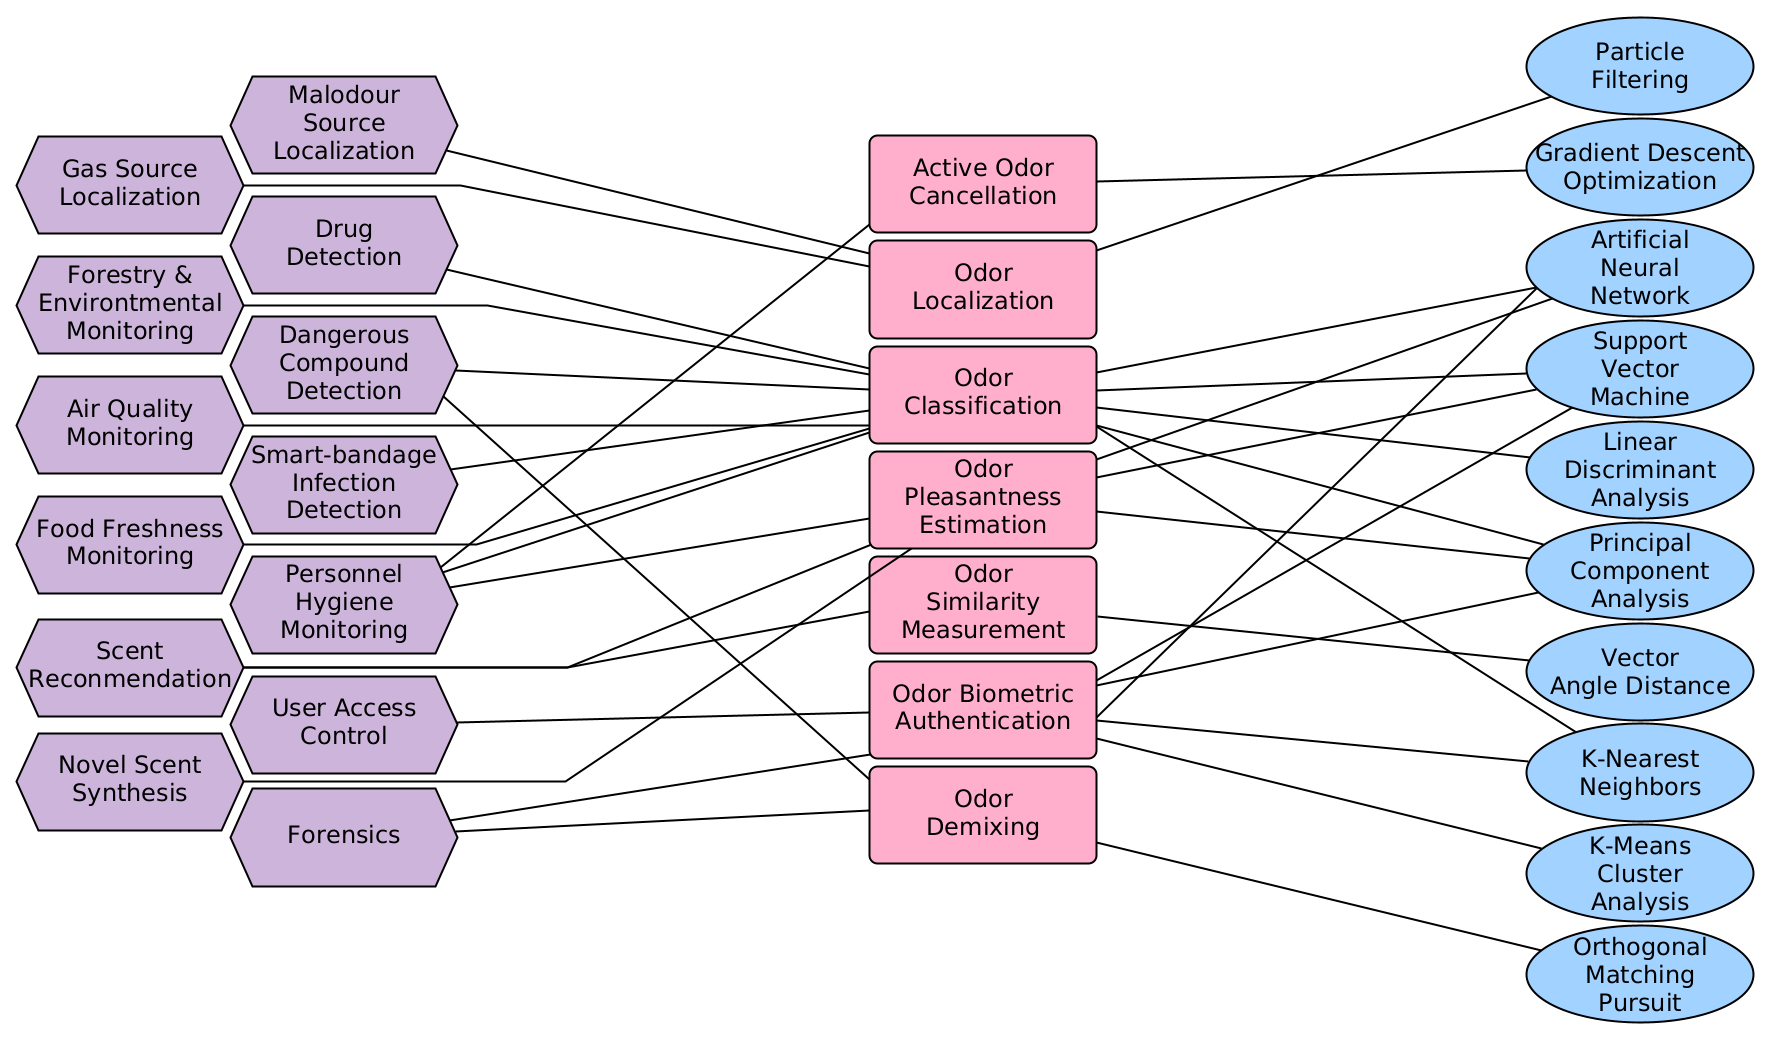
\includegraphics[width=\linewidth]{./figs/app_task_kernel.png}
    \caption{
        \small Graphical depiction of relationship between applications
        (\textcolor{purple}{hexagons}) which are composed from tasks
        (\textcolor{pink}{rectangles}).  Tasks are implemented using a
        computational kernel (\textcolor{blue}{ellipses}). Some tasks can be
        supported by multiple kernels.
    }
    \label{fig:app_task_kernel}
\end{wrapfigure}

In many
domains, the light computational requirements of \olfc{} algorithmic primitives
means the attention of architects is little needed. XR headsets, able to power
high resolution 3D graphics, for example, will have little trouble running
\olfc{} tasks.  However, there are domains with
extreme constraints which make \olfc{} interesting to architects.
Form factors such as wearables, (earrings, pendants, brooches, etc), bandages
(e.g., for detecting infections), adhesives (e.g., for body odor monitoring),
packaging (e.g., smart packages that detect food spoilage), swabs (for breath,
urine, body fluids-based diagnostics, for example), sensors-in-the-wild ( e.g.,
air quality monitoring, surface and ground water quality monitoring), etc., may
only allow for energy harvesting.  Field deployed sensors may need to maximize
limited battery energy capacities over long periods, or be self-powered.  In
these domains, both power and energy are stringent limitations.

 
%Fig.~\ref{fig:arch} presents an overview of \arch{}.
%\arch{}'s aim is to support energy efficient \olfc{}, given the
%lax performance requirements of \olfc{} applications, and the
%constrained energy budget available to edge devices.  Thus, \arch{} is designed
%for operating points at below nominal voltage.

\begin{wrapfigure}{r}{0.5\textwidth}
\centering
    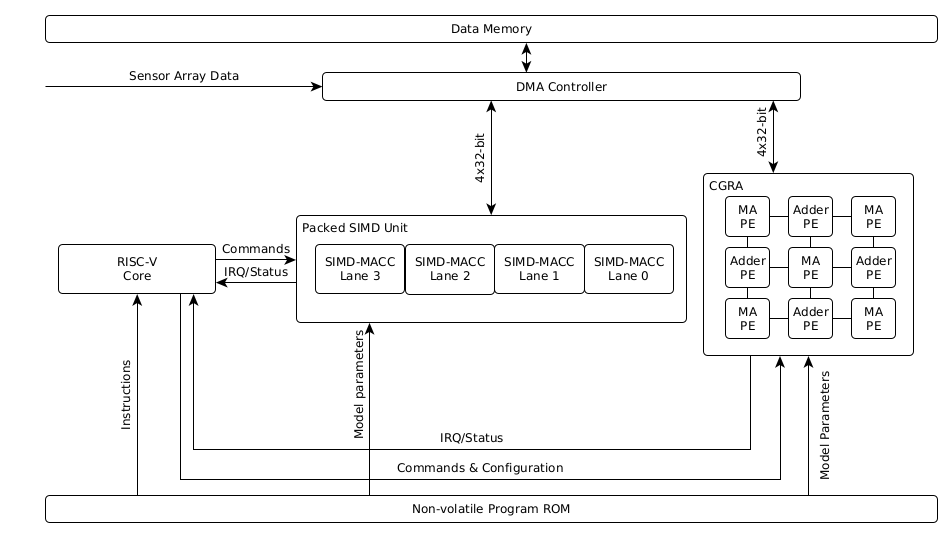
\includegraphics[width=\linewidth]{./figs/odor_arch.png}
    \caption{\small
            Organization of \arch{} as a \mcu{} with \vmacc{} and \cgra{}
            accelerators. Since \arch{} aims for energy efficiency, achieved by
            operating at low voltage and frequency, \arch{} exploits the lack
            of voltage scaling available to SRAMs to enable multiple SRAM
            accesses on a single port per clock cycle.
        }
    \label{fig:arch}
\end{wrapfigure}

Therefore, as a case study, we consider the architecture of a programmable
ultra-low-power \olfc{} hardware platform supporting low frequency
and voltage operation; programmability is supported to lower costs and to
maintain generality in a domain where applications are likely to evolve.  Our
architecture, \arch{} (Fig.~\ref{fig:arch}), is a heterogeneous reconfigurable
odor monitoring and analysis architecture consisting of a \SI{32}{\bit} RISC-V
MCU (RV32IM) with two integrated accelerators, both supporting fixed-point
operations. The \mcu{} is a four-stage, in order, scalar core based off of the
Open Hardware Group's CORE-V CV32 RISC-V IP~\cite{CV32_RISCV_IP}.  \arch{}
can be used to support \olfc{} systems, as in Fig.~\ref{fig:man_vs_machine}.

The first accelerator is a \SI{128}{\bit} packed SIMD unit which accelerates
fixed-point fused muliply accumulate operations on 4, 8, 16, and \SI{32}{\bit}
datatypes, to support the copious multiply-accumulates found in ANN, SVM,
LDA, PCA, VAD, and OMP algorithms.
Unlike a typical packed SIMD ISA extension, \arch{}'s \vmacc{} does not have an
additional SIMD register file.  Instead, data is accessed directly from memory,
which is made possible by the discrepancy between the core voltage at the
minimal energy operating points of \arch{} (Section~\ref{sec:results}), and the
SRAM's nominal voltage required to ensure memory retention. Additionally,
since the size of data memory required by many applications (Table~\ref{tab:kernels})
is small, the overhead of a dedicated SIMD register file may be large relative
to data memory in its entirety
(this is explored further in Section~\ref{sec:results}, where data memory is
replaced/augmented with a flip-flop based register file).

In order to exploit
data reuse found in linear algebraic workloads (i.e., mapping a sequence of
vectors by the same linear transformation), the \vmacc{} contains a buffer
which can be loaded with model parameters, or sensor data, neural network
activations, and other runtime data. The second accelerator is a coarse-grained
reconfigurable streaming dataflow architecture with nine heterogeneous PEs
(adder PEs, and multiply-accumulate PEs) arranged in a \(3\times 3\) grid, and
utilizing a bufferless, single-cycle, multi-hop routing network, as
in~\cite{wang2019hycube, gobieski2021snafu}. Each PE contains a small
(\SI{16}{\byte}) buffer, in which it can store model parameters, as well as
accumulated sums.  \arch{}'s \cgra{} is based off of the SNAFU low-power
reconfigurable architecture. PEs are capable of \SI{32}{\bit} width packed-SIMD
execution of multiplies and adds (i.e., $1\times$ \SI{32}{\bit} operation,
$2\times$ \SI{16}{\bit} operations, etc.).  The dataflows supported  on
the CGRA enables mapping convolution layers with various kernel sizes and strides.
This is important as although currently most \olfc{} ANNs are MLPs,
there do exist CNNs for \olfc{} applications, and the choice of the best
model for \olfc{} tasks is still being litigated.

Both accelerators support efficient packed SIMD addition and multiplication for
datatypes of varying width, as wide adders and multipliers can be
recursively built from narrow adders and multipliers.
Wide adders are built from narrow adders via carry-out propagation.
Wide multipliers are built from narrow multipliers via convolution
(or, polynomial multiplication), as in Fig.~\ref{fig:poly_mul}.
This figure shows how narrow multipliers can be used to compute partial
products for a wider multiplier (Fig.~\ref{fig:poly_mul_pp}).
These partial products are then summed
to generate wider multiplier's product (Fig.~\ref{fig:poly_mul_red}).
When configured to support the `narrow' datatype, the multiplier simply
outputs the \(A_1B_1\) and \(A_0B_0\) products, while when configured
to support the `wide' datatype, the multiplier outputs the full \(AB\)
product.  This technique can be recursively applied, which enables
\SI{8}{\bit}, \SI{16}{\bit}, and \SI{32}{\bit} multipliers to all be built
from \SI{4}{\bit} multiplier primitives.
Note that when operating on the `narrow` datatype, there are twice as many
partial product generating multipliers as required.  These multipliers can
be clock-gated, reducing dynamic power consumption in the multipliers and
the adder reduction tree.  A second use for these multipliers could be to increase
the total width of the packed SIMD units. However, doing so would require
doubling the data memory bandwidth.  At ultra-low frequency operating points,
this may be possible, however, it is not explored in \arch{}.
In fixed-point arithmetic, shifters are used to rescale products.
These are implemented for the different datatypes in parallel, and the output
is muxed based on the datatype required. In both the \vmacc{} and the \cgra{}
PEs, the multipliers are pipelined to ensure they meet timing at nominal
voltage and frequency.  Exact location of pipeline registers is determined by
register retiming.
To support ANNs, both accelerators are programmed to perform either linear or
reLU activations on accumulated data before writing the results to data memory.

\begin{wrapfigure}{l}{0.5\linewidth}
\centering
\begin{subfigure}{\linewidth}
    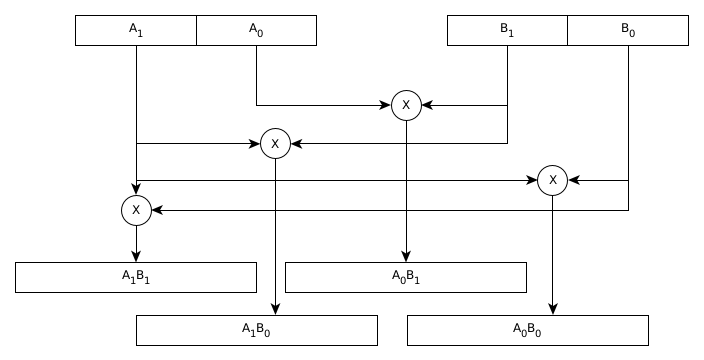
\includegraphics[width=\linewidth]{./figs/poly_mul.png}
    \caption{Partial product computation.}
    \label{fig:poly_mul_pp}
\end{subfigure}

\begin{subfigure}{\linewidth}
    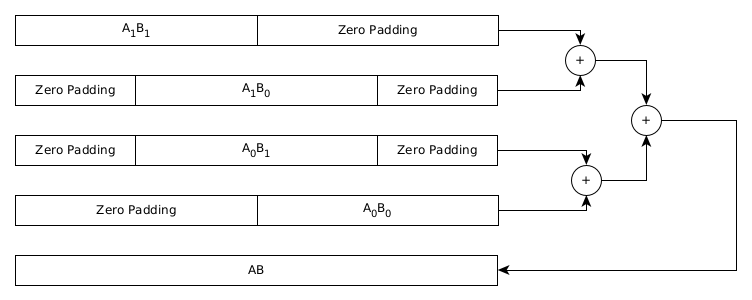
\includegraphics[width=\linewidth]{./figs/poly_mul_reduction.png}
    \caption{Partial product reduction.}
    \label{fig:poly_mul_red}
\end{subfigure}
\caption{Narrow multipliers are converted into wider multipliers via
convolution, or polynomial multiplication.}
\label{fig:poly_mul}
\end{wrapfigure}

The accelerators are given direct access to data memory, which enables the
\mcu{} to be idle while the accelerators work.  The accelerators signal
completion of their work via IRQ lines.  The core can also choose to poll the
accelerator's status register if the accelerator is expected to finish its task
quickly.  Since accelerator launch costs are small (due to the small size of
the CGRA, and small number of operations supported by both architectures), and
the often large number of linear operations between non-linear operations
(Table~\ref{tab:kernels}), the accelerators are focused on accelerating linear
operations, and specifically fused multiply-accumulates.  This means that
non-linear operations are left for execution on the \mcu{}.

\arch{}  uses a modified Harvard architecture, in which program instructions
and model parameters are stored in a non-volatile ROM, while read-write data
is stored in an SRAM-based data memory.  Since standard SRAMs cannot be safely
voltage scaled without error detection and correction coding~\cite{kumar2009sram}, a single
SRAM bank may be accessed multiple times by the DMA controller in each compute
clock cycle.

\arch{} may be run in one of three modes.  In MCU mode, only the \mcu{} is
active, with both accelerators powered off. In MCU+SIMD mode, the \mcu{} and
\vmacc{} are used, but the \cgra{} is powered off.  In MCU+CGRA mode, the
\mcu{} and \cgra{} are powered, while the \vmacc{} is powered off. Which mode
to use in deployment is determined statically by the programmer after analyzing
performance in the different modes.

\begin{figure*}[h]
    \centering
    \begin{subfigure}{0.3\textwidth}
        \centering
        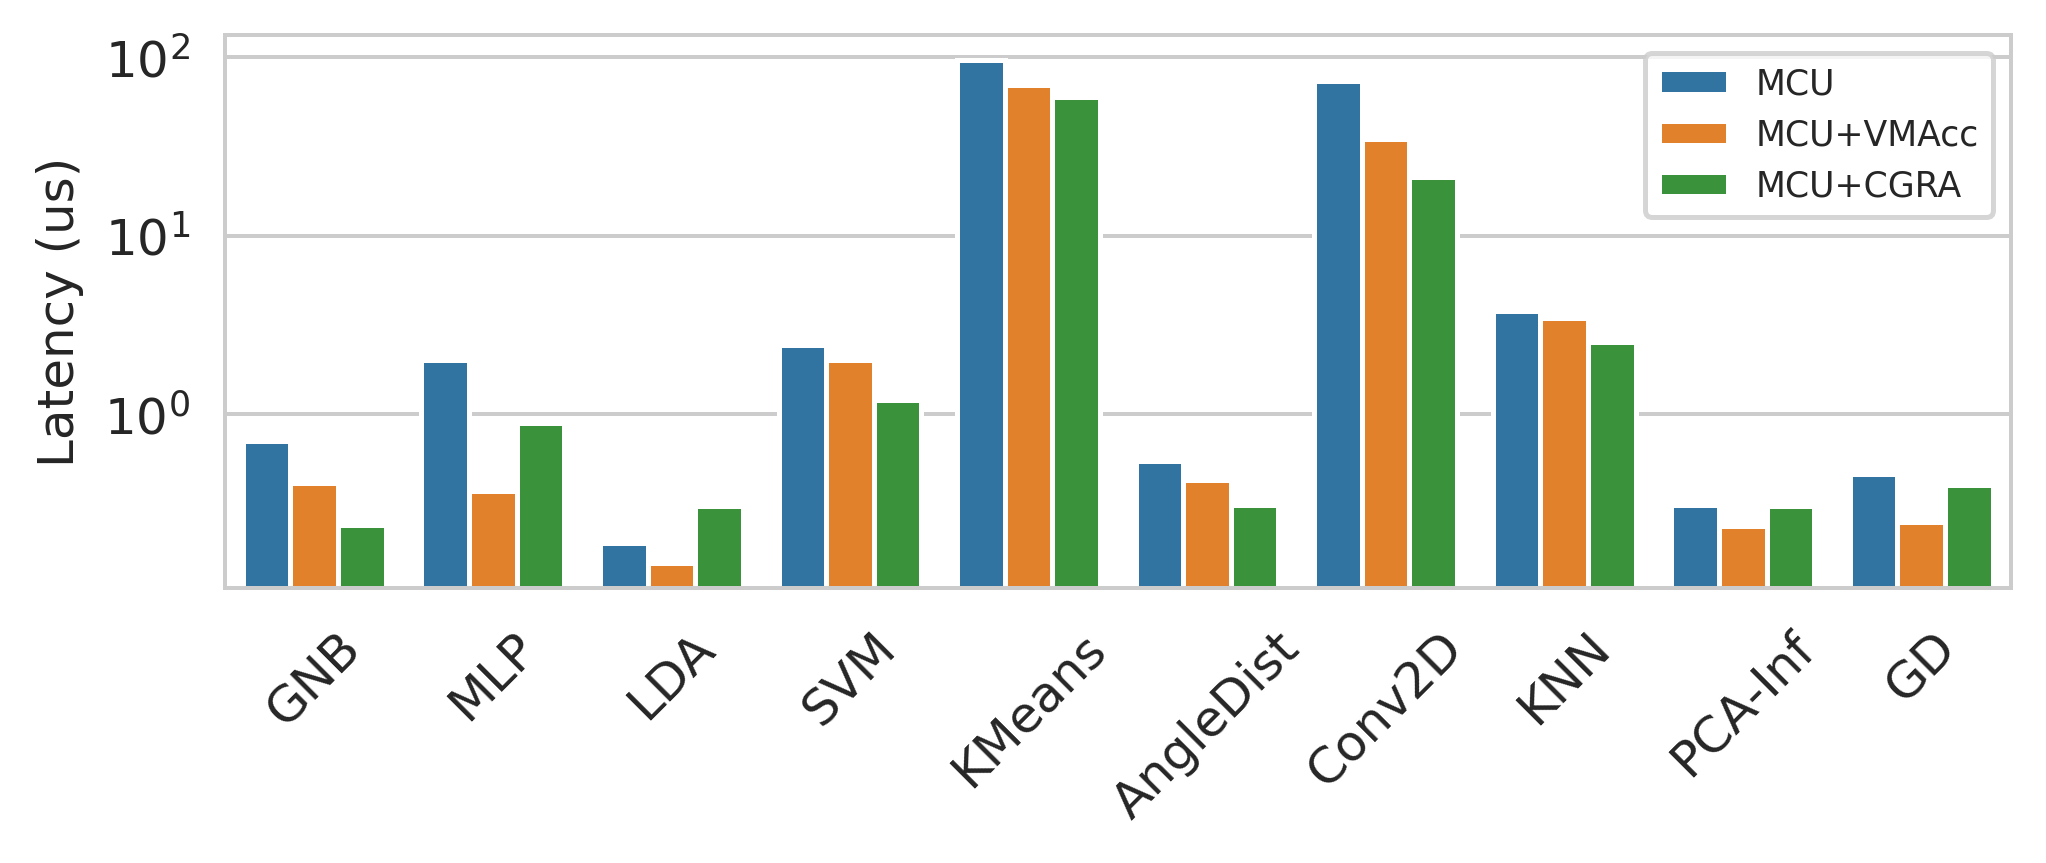
\includegraphics[width=1.0\linewidth]
            {./figs/one_volt_latency.png}
        \caption{\small Performance of \arch{}'s modes across benchmarks.}
        \label{fig:baseline_latency}
    \end{subfigure}
    \begin{subfigure}{0.3\textwidth}
        \centering
        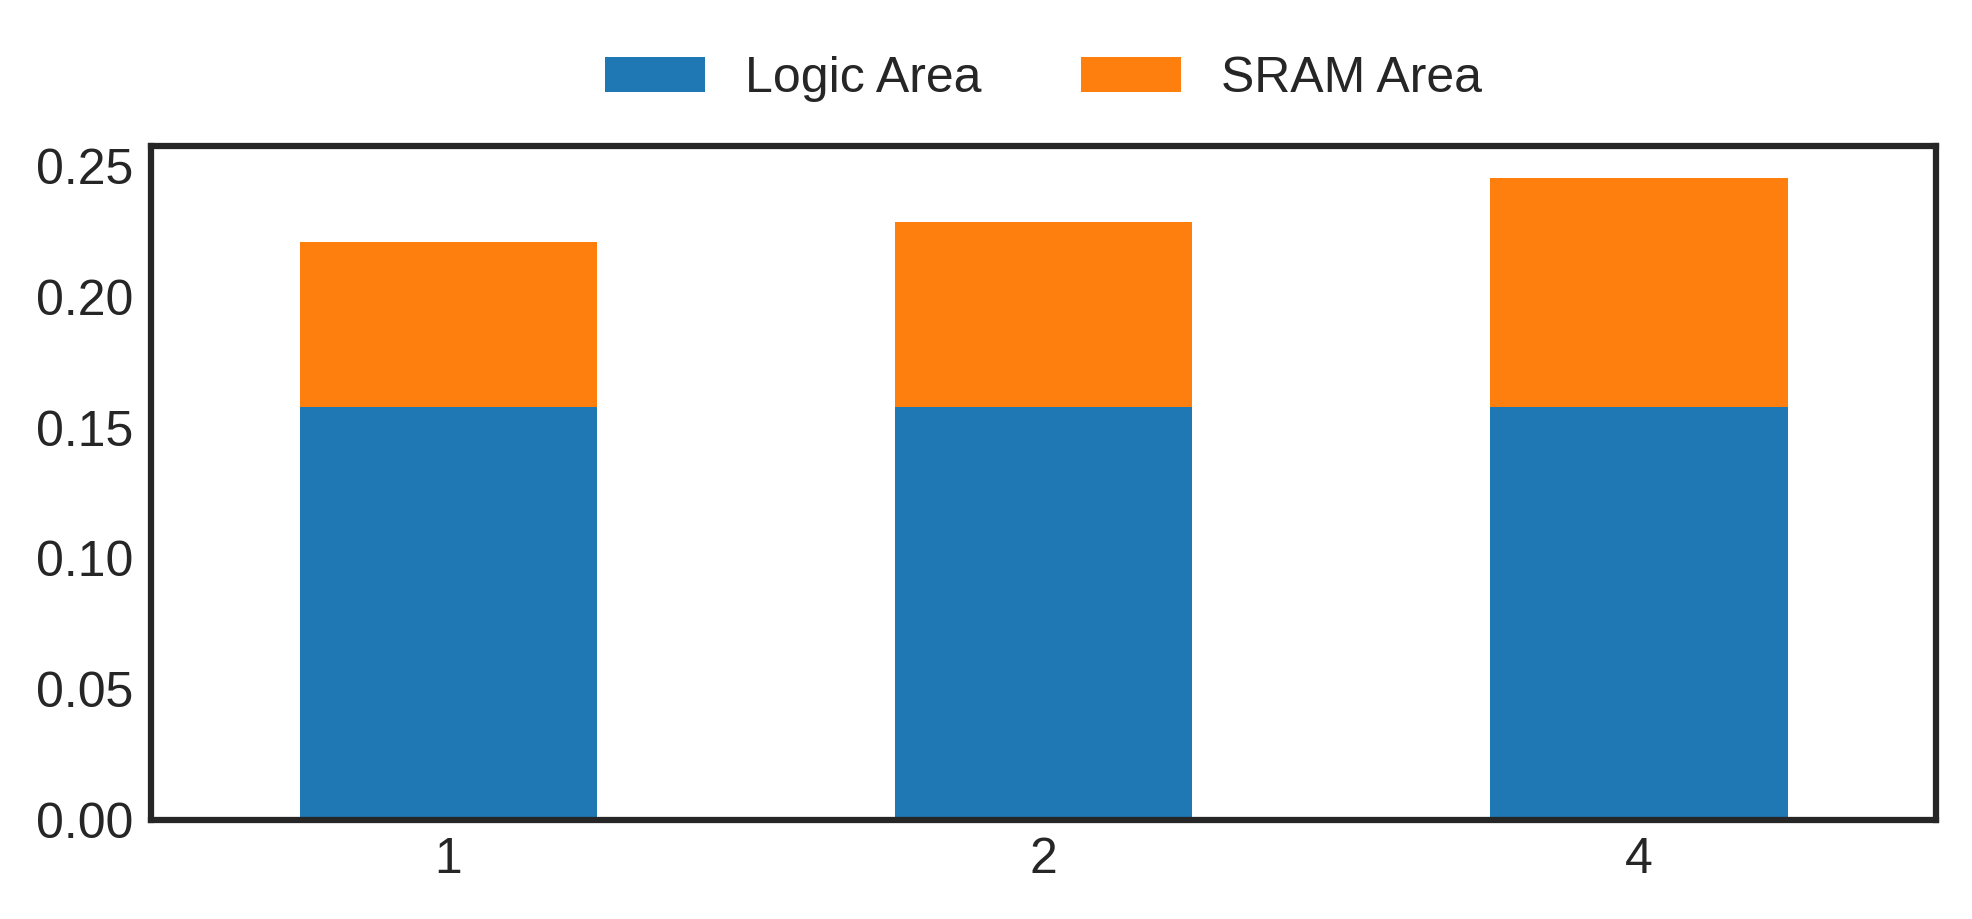
\includegraphics[width=1.0\linewidth]
            {./figs/one_volt_area.png}
        \caption{\small Area needed to support \arch{}'s modes with
            SRAM organized into one, two, and four banks.
        }
        \label{fig:baseline_area}
    \end{subfigure}
    \begin{subfigure}{0.3\textwidth}
        \centering
        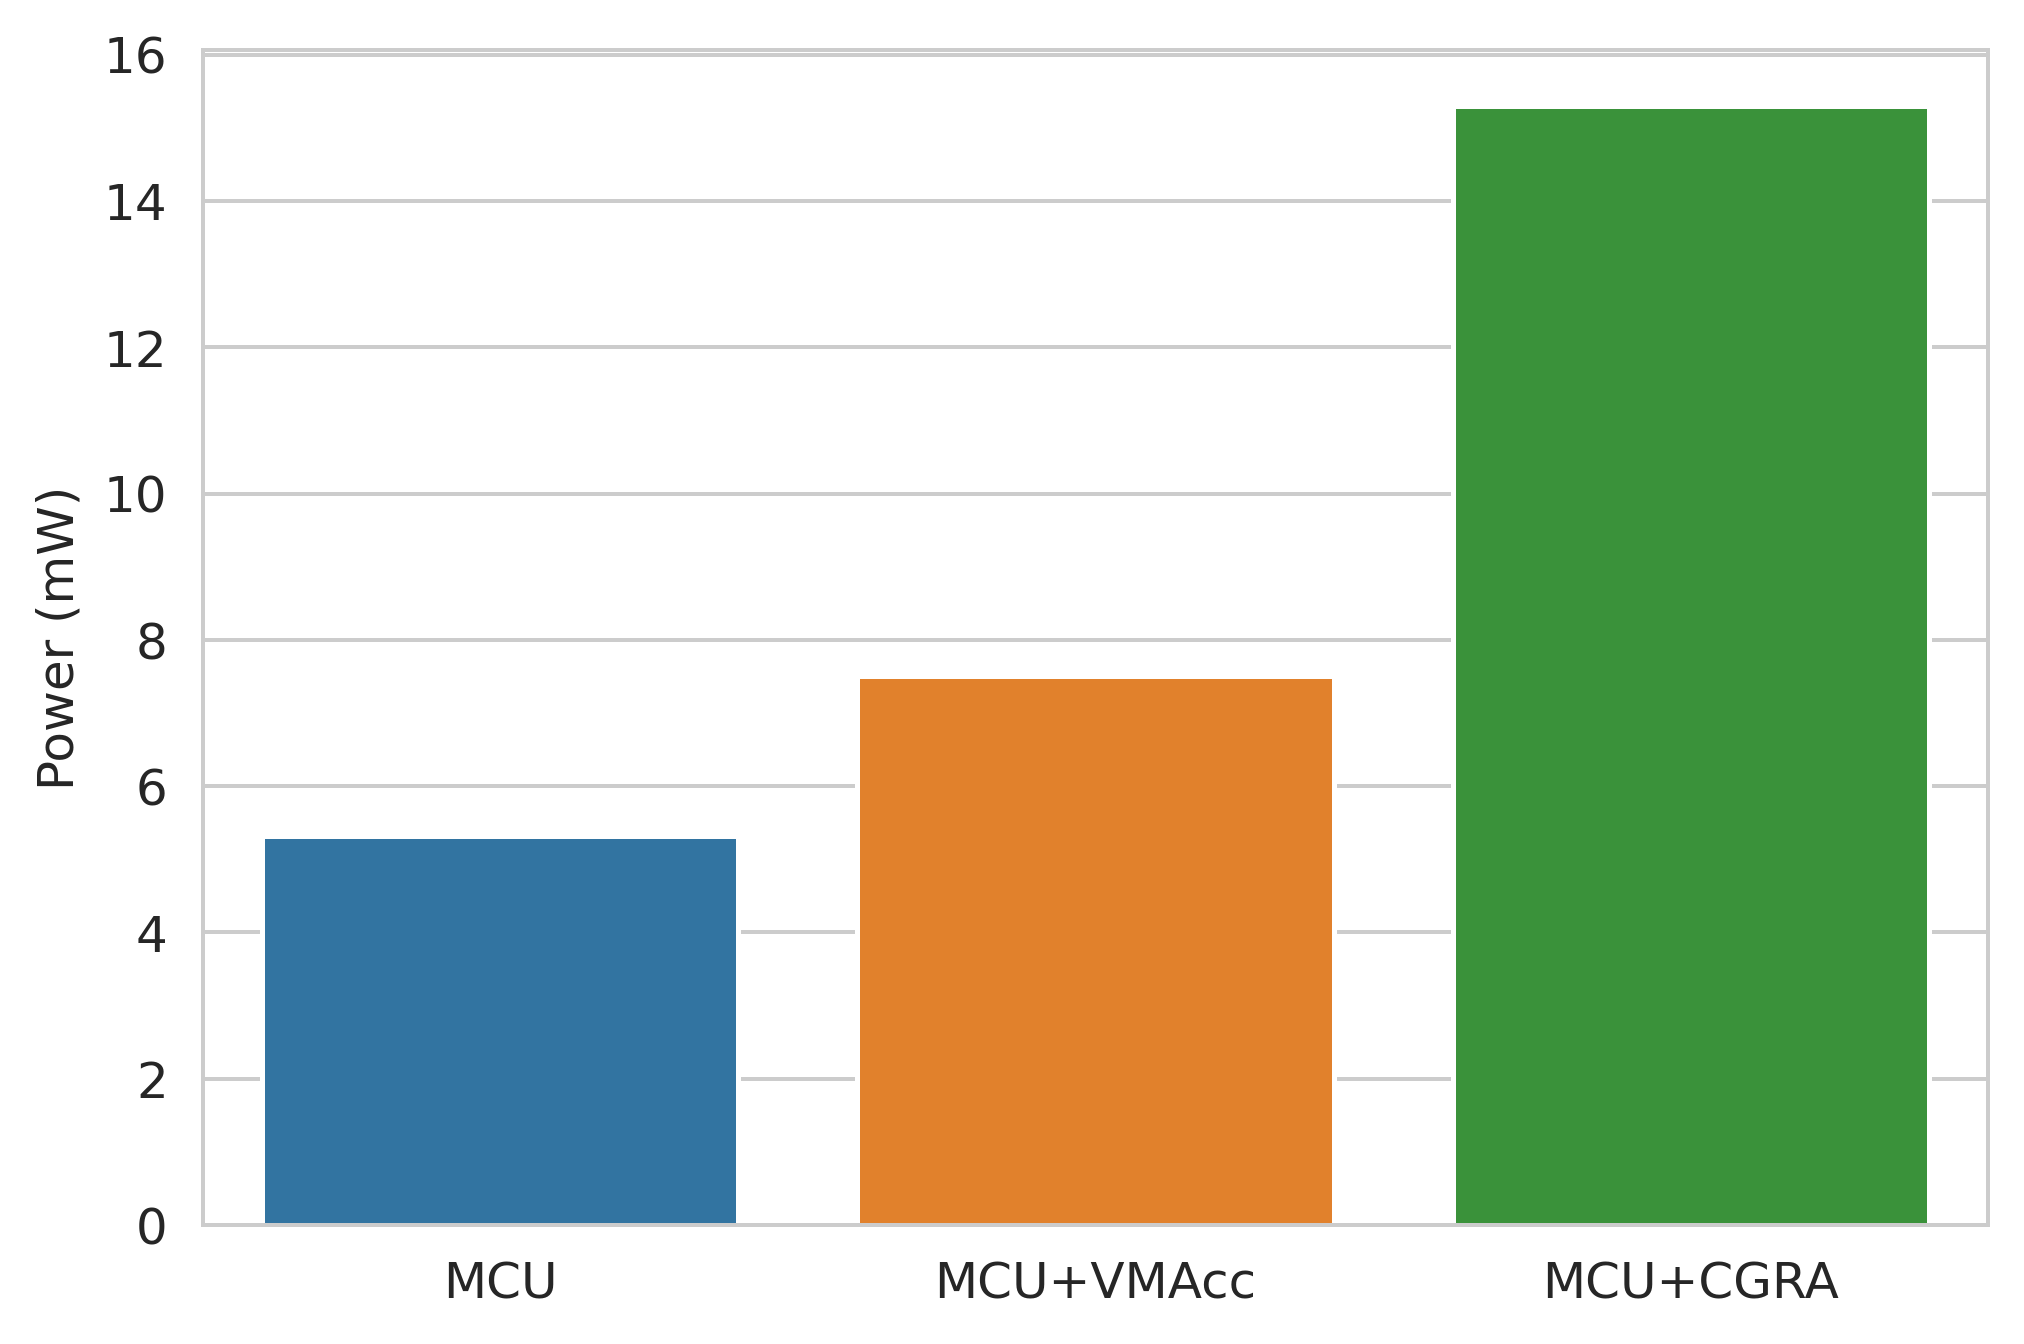
\includegraphics[width=1.0\linewidth]
            {./figs/one_volt_power.png}
        \caption{\small Power consumption of \arch{}'s modes.}
        \label{fig:baseline_power}
    \end{subfigure}
    \\
    \begin{subfigure}{\linewidth}
        \centering
        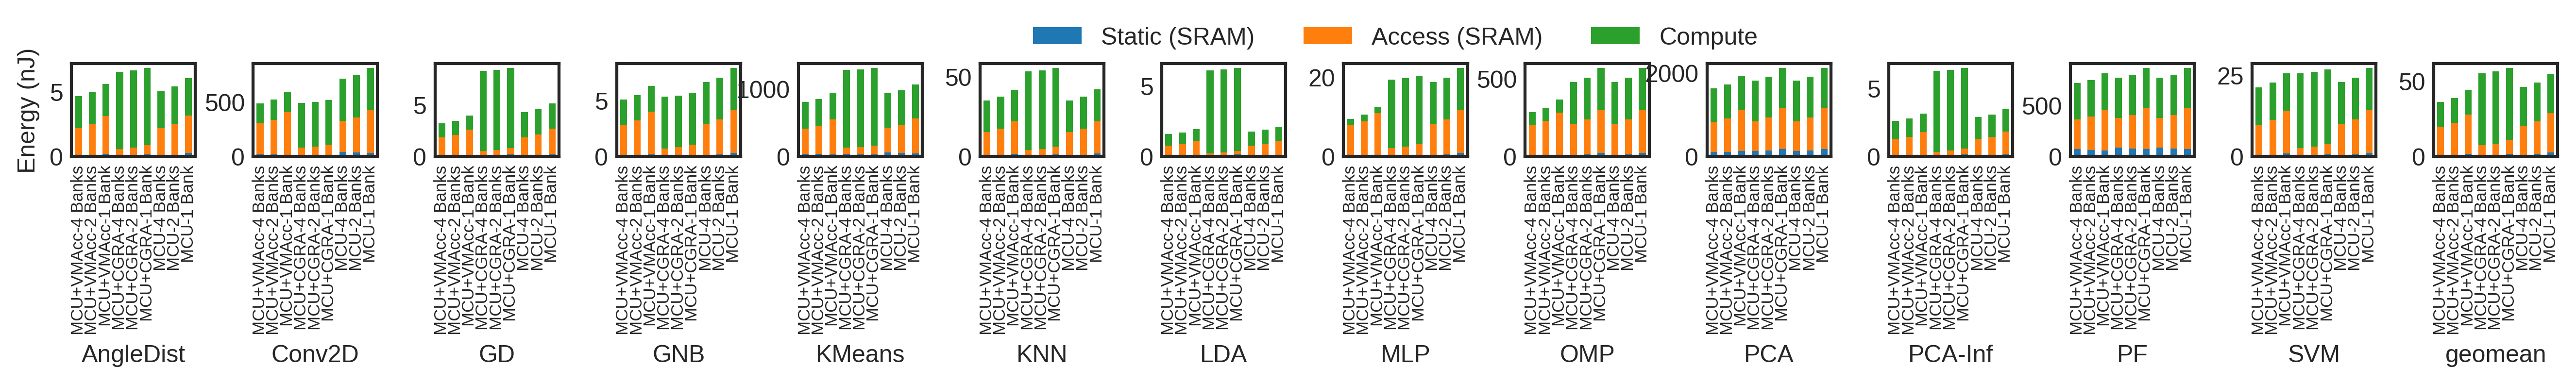
\includegraphics[width=1.0\linewidth, height=0.25\textwidth]
            {./figs/one_volt_total_energy.png}
        \caption{\small Total energy consumption of \arch{}'s modes
        for each kernel and with several SRAM organizations.}
        \label{fig:baseline_energy}
    \end{subfigure}
    \caption{\small Baseline Results.}
    \label{fig:baseline_results}
\end{figure*}


Fig.~\ref{fig:baseline_results} shows baseline results for \arch{} with several
SRAM organizations at nominal frequency (\SI{600}{\mega\hertz}) and voltage
(\SI{1}{\volt}). \arch{}'s performance on the kernels is shown in
Fig.~\ref{fig:baseline_latency}, broken down by \arch{} mode of operation.
Across all kernels, the mode with the \vmacc{} consistently outperform
the \mcu{} baseline (Fig.~\ref{fig:baseline_latency}). Similarly, for most
kernels, the \cgra{} based mode outperforms the \mcu{} baseline.
However, for applications with very small amounts of compute (e.g., LDA), the
CGRA configuration and launch overhead offset the speed-up provided by the
CGRA, resulting in faster execution on the \mcu{} alone. Despite this, the CGRA
is the best performer on a number of benchmarks, including Conv2D - a kernel
vital in CNNs, and SVM. The high performance of the parallel architectures is
due to the prevalence of multiply-accumulates within the kernels, as discussed
in Section~\ref{sec:workloads}.

The same pattern also emerges for energy (Fig.~\ref{fig:baseline_energy}), with
mode with the MCU+SIMD outperforming the MCU alone in energy efficiency, while
the MCU+CGRA only outperforms the MCU on several kernels and outperform the
MCU+SIMD on Conv2D, due to the high power consumption of the MCU+CGRA. The
figure also shows the importance of using multiple SRAM banks. By dividing the
SRAM into banks, banks which are unneeded for a given application kernel may be
put into retention mode, eliminating nearly all power consumption of the SRAM.

Fig.~\ref{fig:high_power_energy_banking} shows the absolute energy consumed by
\arch{}'s modes at their minimal energy operating point (MEOP) on a
\SI{10}{\milli\watt} nominal power budget.  The MEOPs are \SI{0.4}{\volt} and
\SI{357}{\mega\hertz} for the MCU and and MCU+SIMD, and \SI{0.4}{\volt} and
\SI{119}{\mega\hertz} for the MCU+CGRA. Operating at the MEOP provides
significant energy efficiency improvement over the nominal operating point due
to reduction in dynamic power which decreases superlinearly with reduction in
frequency. This can be seen by the growth in the proportion of energy consumed
by SRAM reads and writes, relative to Fig.~\ref{fig:baseline_energy}. Operating
at MEOP enables the MCU+CGRA to become the most energy efficient mode on most
kernels, with MCU+SIMD being the most energy efficient on OMP and PF. On
average, the MEOP provides \MeopImprovementMcu{}, \MeopImprovementVMAcc{}, and
\(\MeopImprovementCgra{}\times\) improvement over the nominal operating points
for the \mcu{}, \mcu{}+\vmacc{}, and \mcu{}+\cgra{} modes, respectively.

\begin{figure*}[tb]
    \centering
    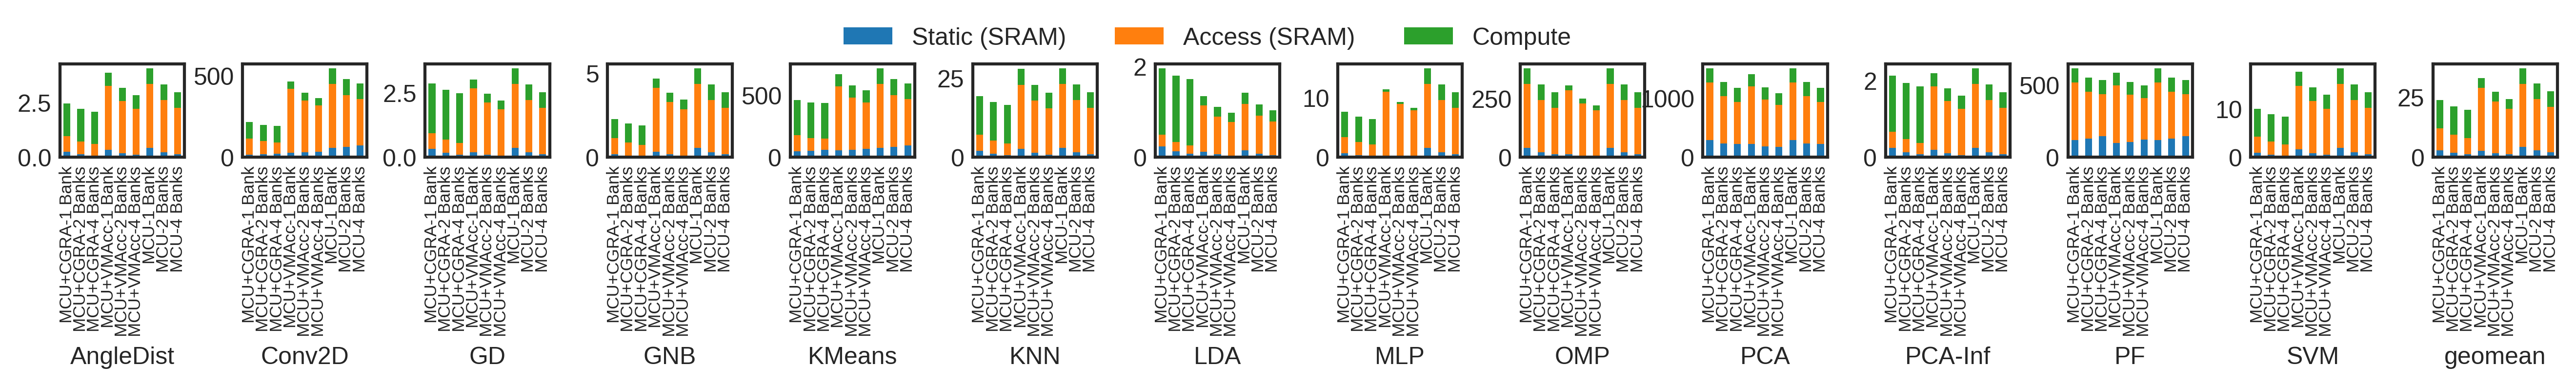
\includegraphics[width=1.0\linewidth]{./figs/high_power_energy_banking.png}
    \caption{\small
        Energy consumption at the MEOP on each kernel with different SRAM
        organizations: One 2048 word SRAM, two 1024 word SRAMs, and four 512
        word SRAMs.
    }
    \label{fig:high_power_energy_banking}
\end{figure*}

% \input{./tables/mass-data.tex}
% Table~\ref{tab:mass-data} contains details of energy breakdowns for each
% kernel in each \arch{} mode for several SRAM organizations at the minimal
% energy operating point.

\begin{wrapfigure}{l}{0.5\linewidth}
    \centering
    \begin{subfigure}{\linewidth}
        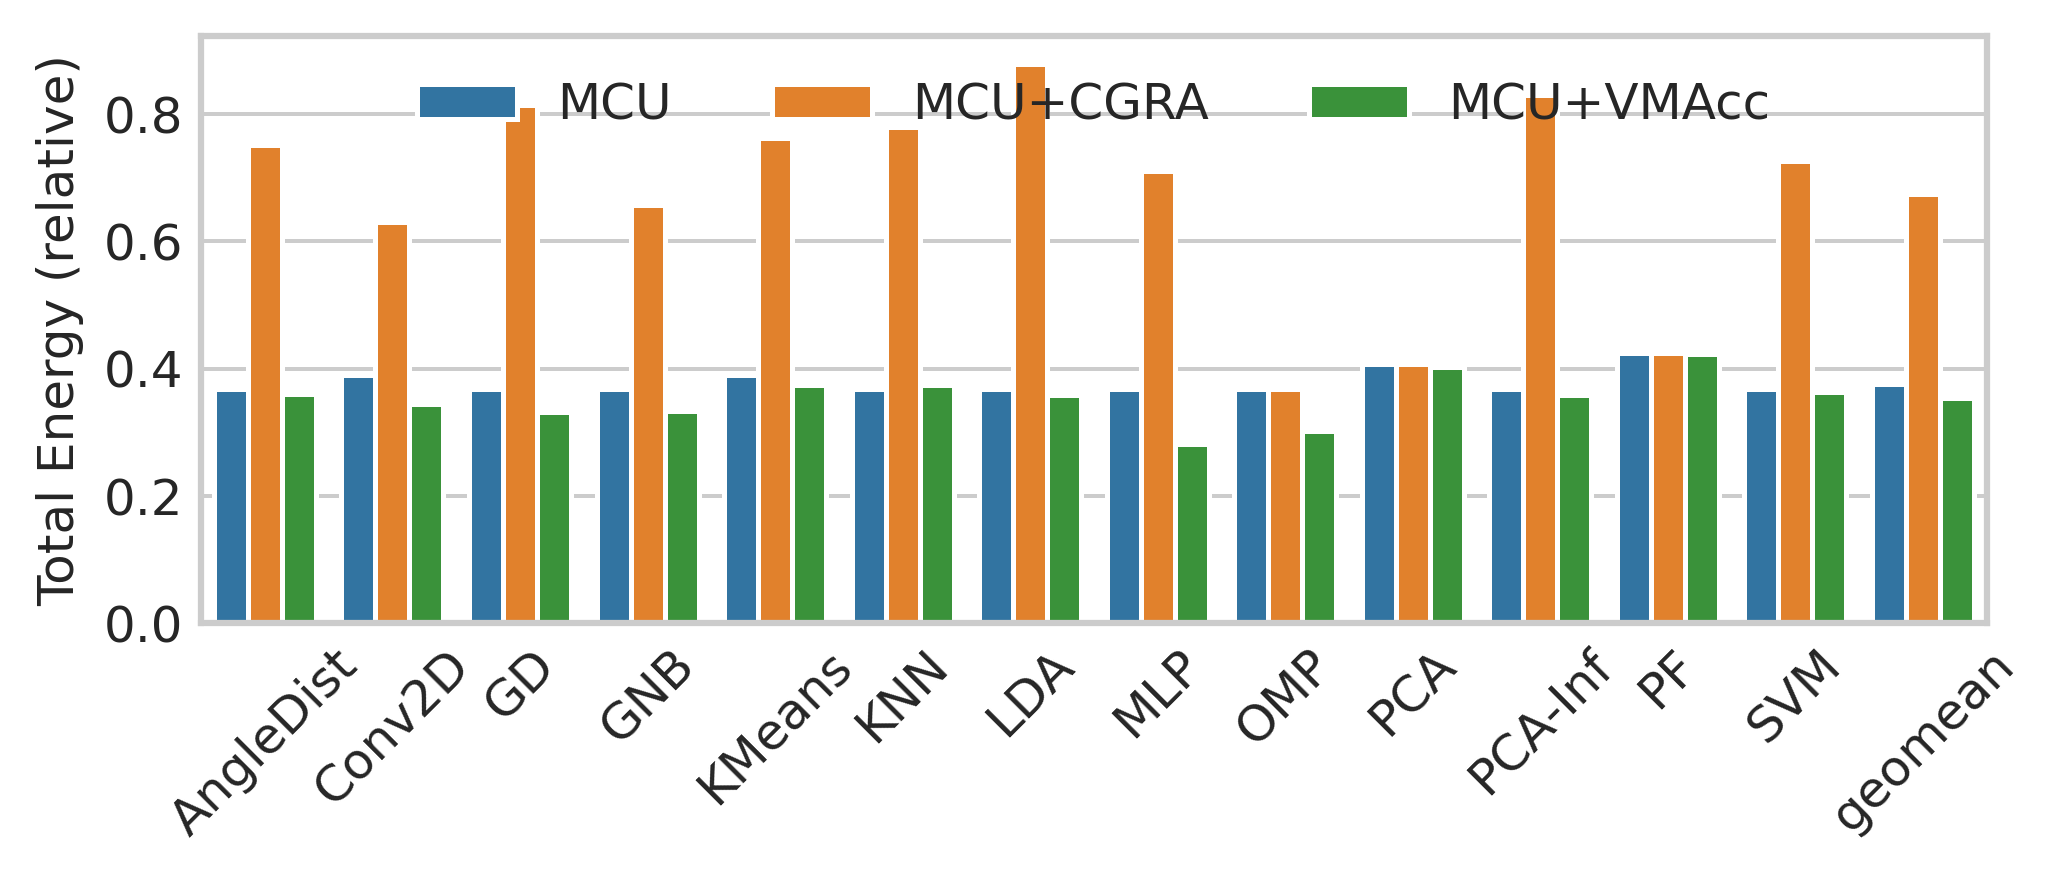
\includegraphics[width=1.0\linewidth]
            {./figs/4KB_tech.png}
        \caption{
            \small Energy achieved at MEOP for \arch{}'s modes across kernels
            with \SI{4}{\kibi\byte} memories built out of flip-flops relative
            to execution with a standard \SI{4}{\kibi\byte} SRAM.
        }
        \label{fig:four_kb_tech}
    \end{subfigure}

    \begin{subfigure}{\linewidth}
        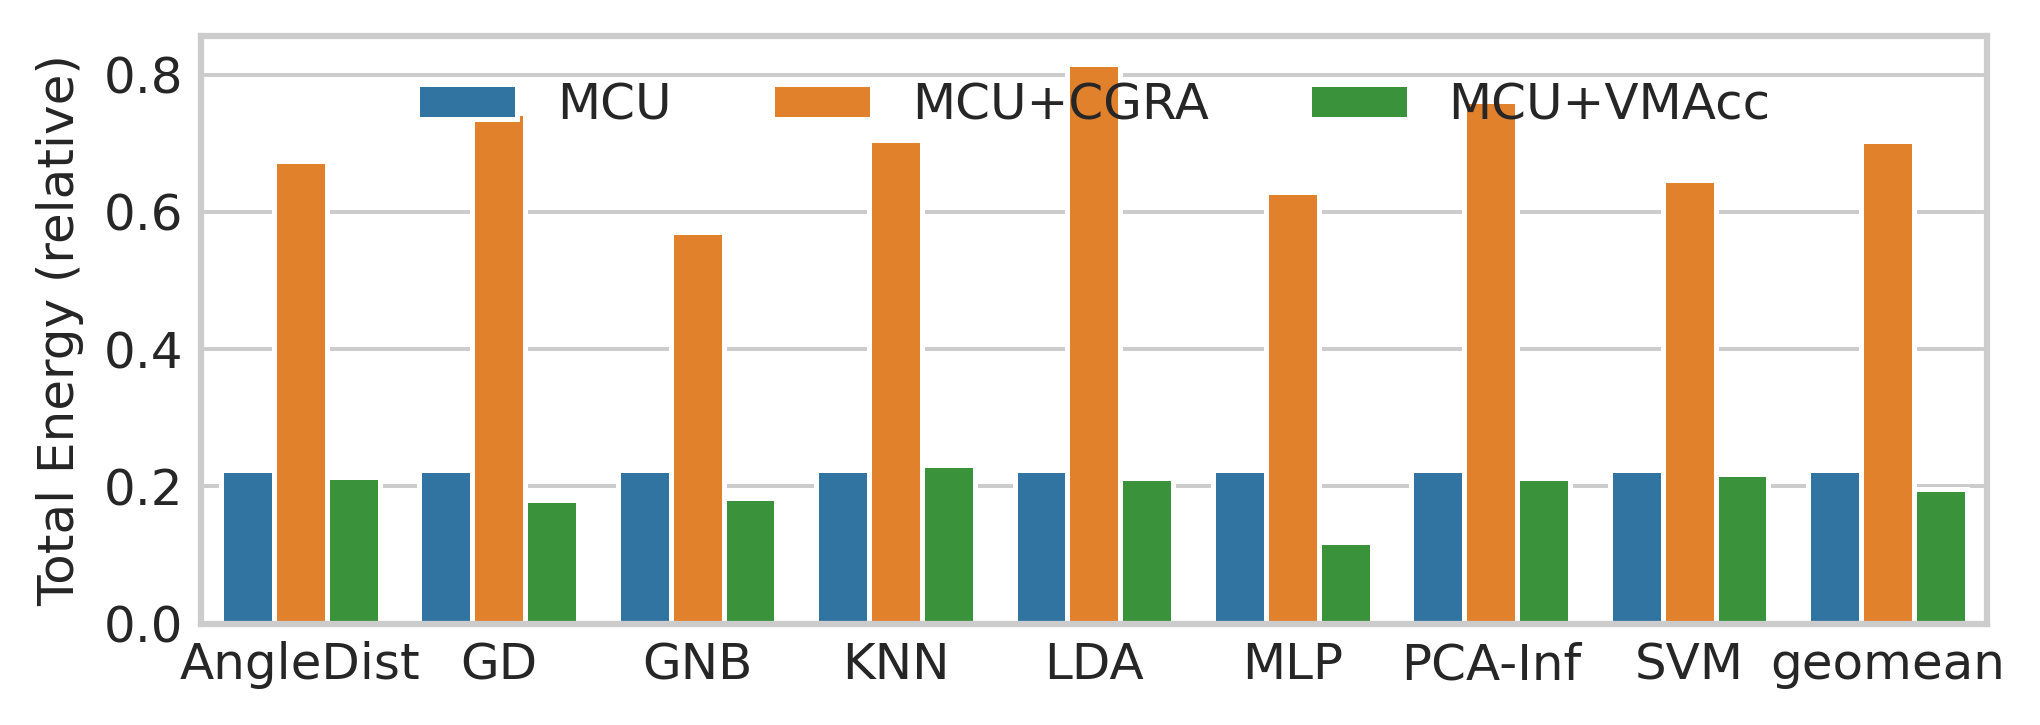
\includegraphics[width=1.0\linewidth]
            {./figs/scratchpad_energy.png}
        \caption{
            \small Energy achieved at MEOP for \arch{}'s modes across kernels
            with a 64-word memory built out of flip-flops relative to
            execution with a standard \SI{4}{\kibi\byte} SRAM.
        }
        \label{fig:scratch_tech}
    \end{subfigure}
    \caption{Replacing SRAMs with flip-flops has a dramatic effect on
    total energy consumption for some of \arch{}'s modes of operation.}
    \label{fig:sram_ff}
\end{wrapfigure}

Fig.~\ref{fig:sram_ff} shows the effects of replacing SRAM with 
memories built out of flip-flops.
In Fig.~\ref{fig:four_kb_tech}, the entire \SI{4}{\kibi\byte} SRAM is replaced
by an equivalently sized memory built from flip-flops.  This enables voltage
scaling to be applied to the memory, whereas with a standard 6T-SRAM, scaling
voltage down to the core's MEOP would likely result in data corruption. The
effects of this are very positive for the MCU and MCU+SIMD modes, both
seeing an over 60\% decrease in energy consumption. In
these modes, SRAM access energy dominates energy consumption.  Thus, the lower
energy of the flip-flop accesses leads to significant energy efficiency
improvements.  This comes despite the fact that the voltage-scaled memory
inhibits the MCU+SIMD from operating at full throughput, due to voltage scaling
of the flip-flop memory leading to increased access latencies. This fact also
mitigates the effectiveness of this technique in the MCU+CGRA mode.
Also, in this mode, compute energy, rather than memory access energy, is the
predominant energy consumption.

In Fig.~\ref{fig:scratch_tech}, \arch{}'s memory is replaced by a small
\SI{256}{\byte} flip-flop based memory.  For kernels with limited data memory
requirements (which is the majority of the studied kernels), this memory
organization results in significant (\(> 4\times\)) energy savings in MCU
and MCU+SIMD modes.  Here, once again, the MCU+CGRA mode sees
less improvement in energy consumption due to increased execution latency, and a
smaller proportion of energy consumption being due to SRAM accesses in
the baseline.  Since the small memory consumes far less dynamic and static
power than the \SI{4}{\kibi\byte} memory, the improvement over the baseline
grows, with the MCU+SIMD mode reducing power by over 80\%.
The smaller memory also helps MCU+CGRA mode, which sees a 30\% reduction
in energy consumption.
Across all kernels, this data memory
organization lead to additional \FFImprovementMcu{}, \FFImprovementVMAcc{}, and
\(\FFImprovementCgra{}\times\) improvements in energy efficiency on average.

The energy savings from flip-flop based memories come at a significant area
cost. The area of \arch{} with \SI{4}{\kibi\byte} memory is
\SI{0.53}{\milli\meter\squared}, a 193\% increase over \arch{} with an equally
sized SRAM.
The overhead of adding the \SI{256}{\byte} memory to \arch{}, however, is small.
Using the small memory as a scratchpad, while retaining the standard SRAM
for applications which may require more memory, results in an area increase
of only 10.3\%.
This demonstrates that, in the the low-power \olfc{} domain, the small memory
requirements of algorithms has a major impact on choice of computer
architecture, with significant trade-offs between area (and hence cost)
and energy efficiency.  This trade-off can be mittigated by using hybrid
memories, composed of small capacity, low density, low power memories, and
larger, denser, higher power memories.


\begin{figure}[h]
    \centering
    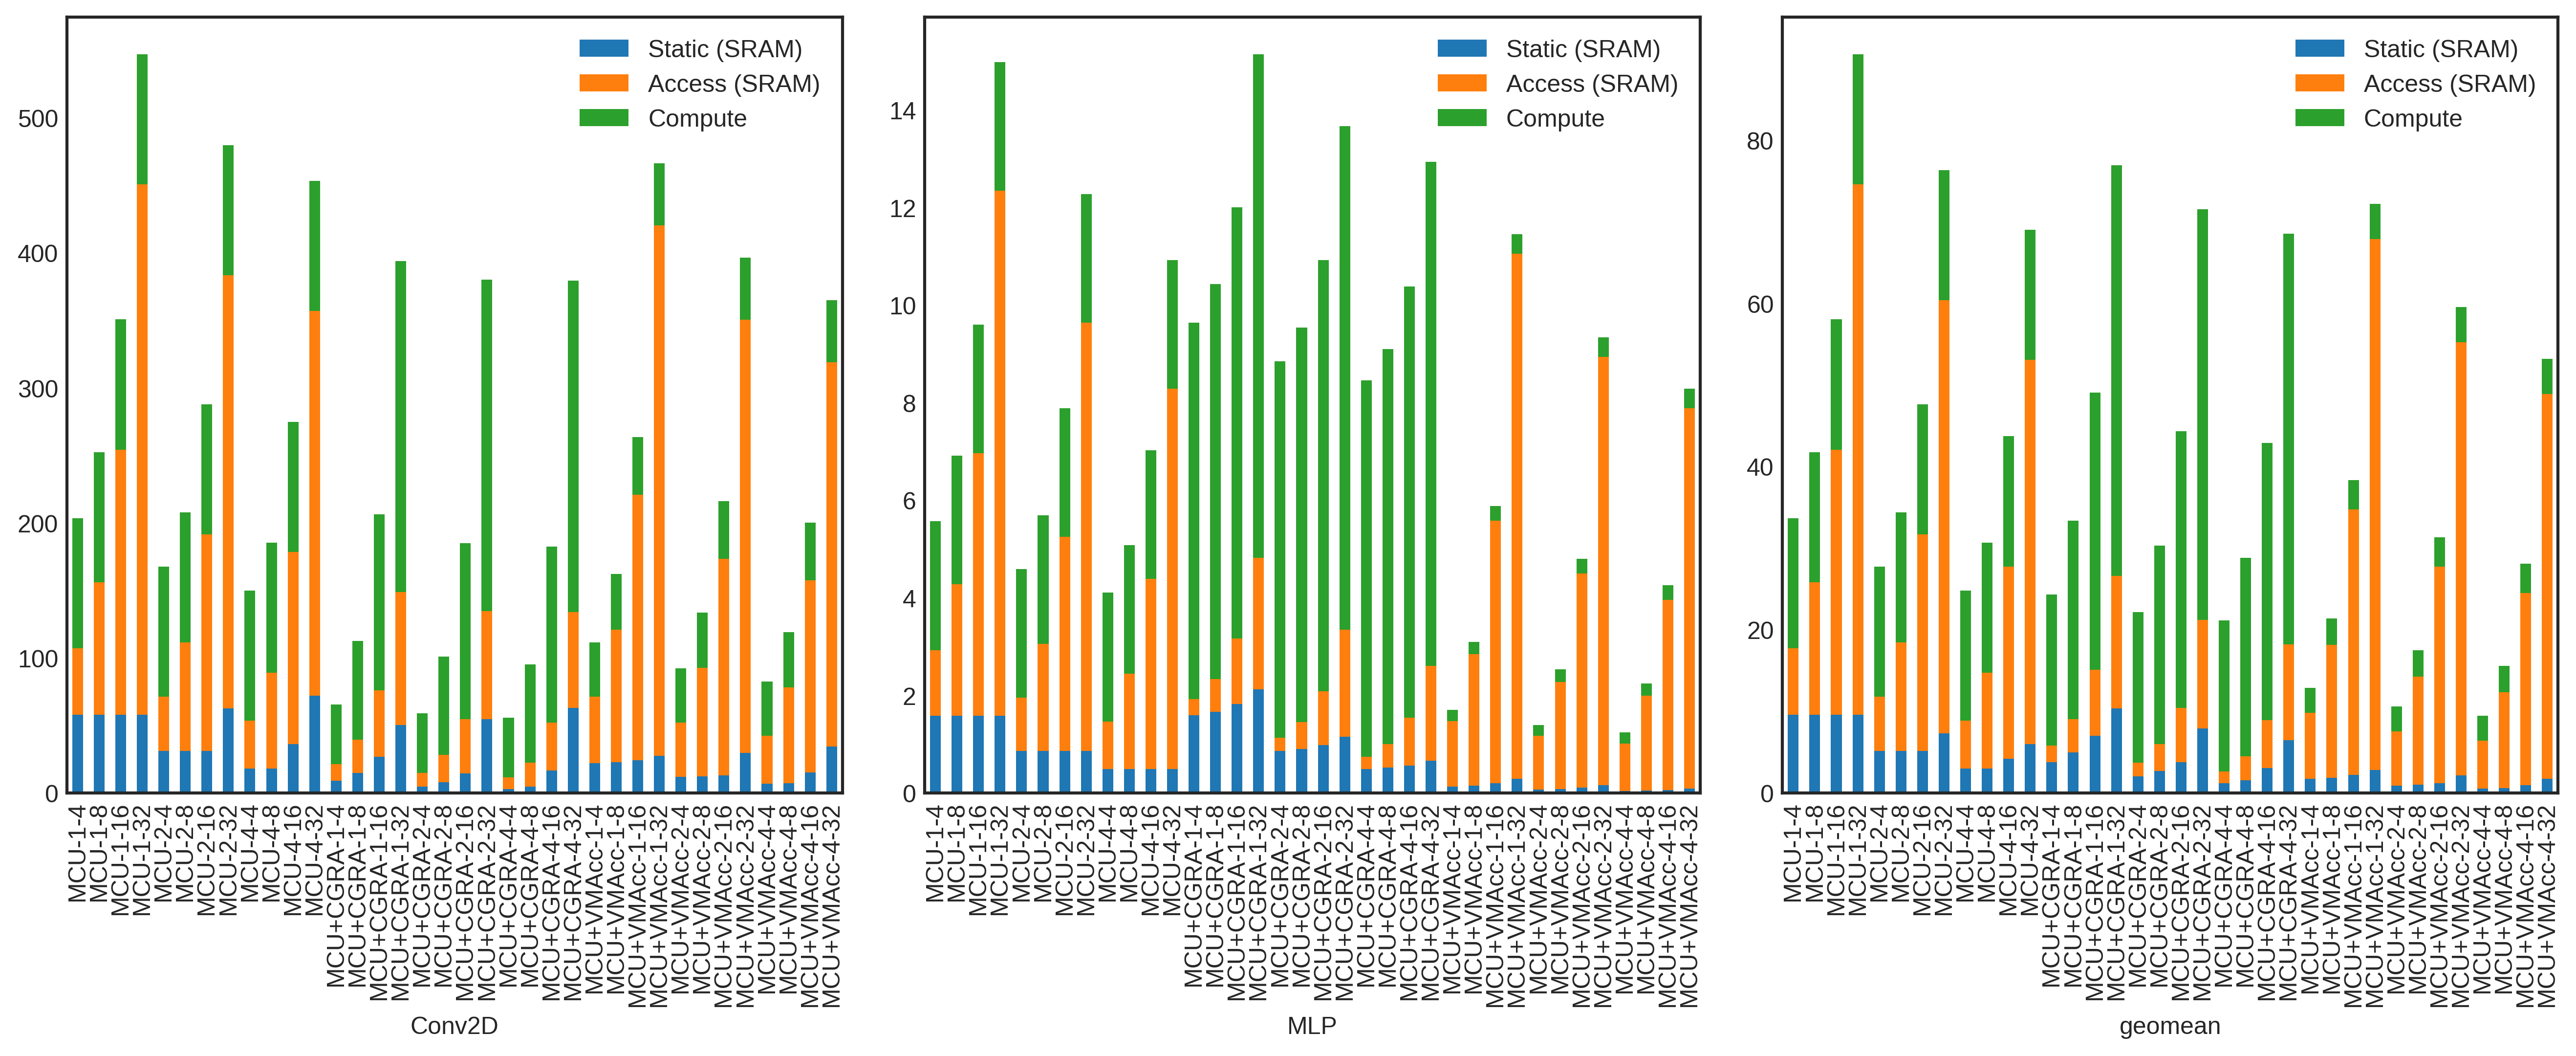
\includegraphics[width=1.0\linewidth]{./figs/high_power_energy_banking_quant.png}
    \caption{\small
        Data quantization leads to decreased energy for appropriate
        kernels.  Further, data quantization's benefits are orthogonal
        to benefits from banking.
    }
    \label{fig:banking_quant}
\end{figure}

%A large corpus of work has demonstrated that the data precision used to encode
%neural network parameters \textit{and} activations can be reduced with
%little impact on classification accuracy~\cite{}.  As such, 
We also evaluate how
parameter and activation quantization impacts energy efficiency in
\olfc{} using the two ANN related kernels (MLP and Conv2D).
Figure~\ref{fig:banking_quant} shows the effects of data quantization
on the architectures at MEOP for a variety of different SRAM organizations.
Benefits for the \mcu{} are the most limited, as the \mcu{} only takes advantage
of quantization through reduction in number of memory accesses.
The \cgra{} and \vmacc{} also see benefit from reduced latency, as they are able to
decrease the latency of the acceleratable portion of the computation via packed
SIMD execution. Packed SIMD execution on multiplies and adds, as is needed
by the \vmacc{} and \cgra{} for the MLP and Conv2D workloads, has negligible
hardware overhead, as word-length multipliers and adders can be built by
recursively composing half-word, byte, and nibble length multipliers
(via convolution) and adders (via carry propagation).
Although not evaluated, the \cgra{} and \vmacc{} could also see decreased
dynamic energy consumption via input gating, as logic used to transform
narrow (e.g., \SI{4}{\bit}) multiplications into wide (e.g., \SI{32}{\bit})
multiplications is not needed when performing quantized operations.
Fig.~\ref{fig:banking_quant} also shows that the improvements from quantization
and from banking are sufficiently orthogonal of one another that 
they can be deployed simultaneously to achieve the effects of both without
interference.

Indeed, there is also a \textit{synergistic} relationship between
banking and quantization, which can be most clearly seen in the Conv2D results
for the \mcu{} mode. In this mode, since performance is independent of both
banking and quantization, when the SRAM bank is available, the amount of
SRAM leakage energy is fixed and independent of quantization.
However, when two banks are used, since quantiztion leads to a decrease
in the total amount of memory required to execute the Conv2D kernel, a single 
SRAM bank may be placed in retention for 4, 8, and \SI{16}{\bit} data, while
both SRAM banks must be active for \SI{32}{\bit} data.  The granularity
of this again increases when four banks are available, with 4 and \SI{8}{\bit}
data types only needing a single bank, while \SI{16}{\bit} data requires
two banks, and \SI{32}{\bit} data requires all four banks.
This same phenomenon plays out with the other modes. However, SRAM leakage
energy in these cases is also impacted by quantization's impact on performance.

\arch{}'s results provide several interesting insights into \olfc{}.
First, when area is not a concern (consider compute area on the back-side of
a solar harvester), a programmable heterogeneous architecture will outperform
monolithic architectures and should be used.  Second, parallel SIMD and dataflow
architectures are effective at improving energy efficiency of even the
very small \olfc{} workloads --- this is not self-evident, as many \olfc{} workloads
have orders of magnitude less compute than even traditional sensor processing.
Third, memory organization has a major impact on energy efficiency in \olfc{},
due to the wide ranging amounts of data memory required by its workloads.


Figure~\ref{fig:vs_baselines} shows how a heterogeneous architecture such as
\arch{} outperforms an an ULP MCU, an ULP MCU with a ULP SIMD unit, and a ULP
CGRA (the individual operating modes of \arch{}, respectively) by
\BaselineGeomeanMcu{}, \BaselineGeomeanVmacc{}, and
\BaselineGeomeanCgra{}$\times$ on average in energy efficiency (in terms of
energy at MEOP). This demonstrates the benefit of our architecture against
possible alternatives.

\begin{wrapfigure}{l}{0.5\linewidth}
\centering
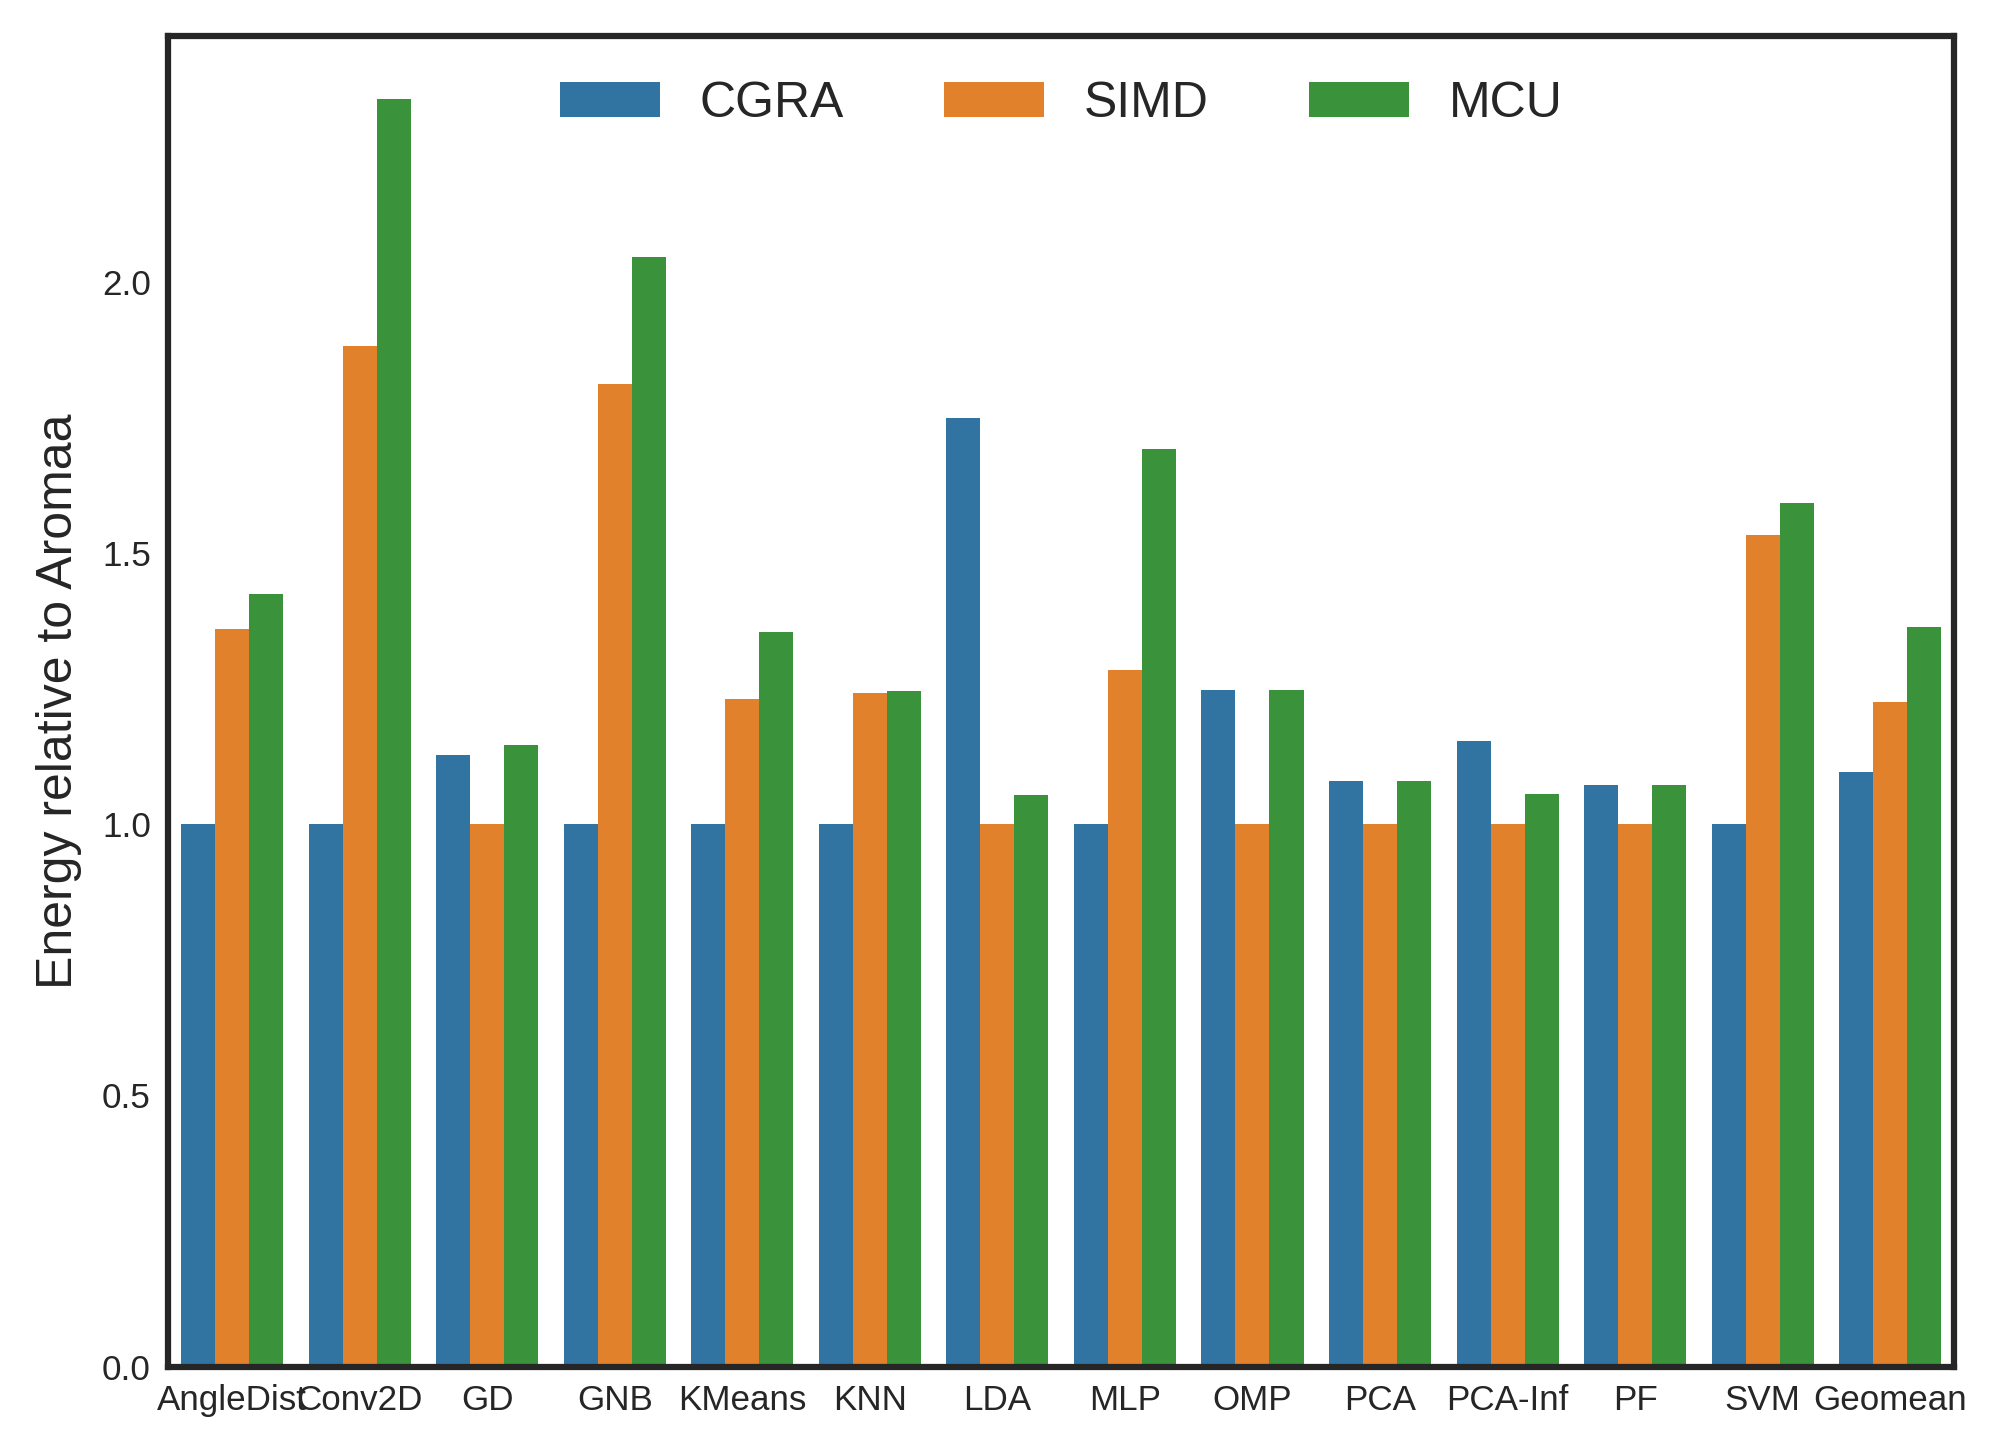
\includegraphics[width=\linewidth]{./figs/comparison_vs_baselines.png}
\caption{\small
    \arch{}'s heterogeneous design allows it to outperform an MCU, an MCU with
    SIMD, and a CGRA baseline in energy efficiency at MEOP.
}
\label{fig:vs_baselines}
\end{wrapfigure}

